\section{Reconstruction of Collision Events in the ATLAS Detector}%
\label{sec:object_reco_at_atlas}

\todo[inline]{Introductory sentence}

Omissions: Photons, special reconstruction techniques for certain analyses


\subsection{Tracking and Vertexing}

The reconstruction of trajectories of charged particles is referred to as track
reconstruction or tracking. The inputs to the track reconstruction in the ID of
the ATLAS detector are \emph{space-points} from the pixel and SCT detector, and
\emph{drift circles} from the TRT. Space-points are measurements of location in
three-dimensional space obtained by clustering the charge signals of adjacent
segments in the pixel and SCT detectors. Drift circles are measurements of
distance from the anode wires of individual straw-tubes in the TRT derived from
electron drift times in the straw-tubes.

Track reconstruction employs pattern recognition techniques to select
space-points and drift circles that are compatible with the hypothesis of a
charged particle in the axial magnetic field of the ID. Least-squares fits are
performed, using selected space-points and drift circles, to determine the
parameters characterising the track at a reference point. This reference point
is typically the point of closest approach (perigee) to the nominal beamspot
position in the transverse plane. Five parameters describe the track at the
perigee. The transverse (longitudinal) distance of the perigee from the
reference point given by $d_0$ ($z_0$), also referred to as the transverse
(longitudinal) impact parameter of the track. The azimuthal and polar angle of
the track at the perigee given by $\phi$ and $\theta$, respectively. Finally,
the ratio of electric charge and transverse momentum, $q / \pT$, parameterises
the curvature of the track.

At the ATLAS experiment, two primary tracking algorithms are used which are
referred to as the \emph{inside-out} and \emph{outside-in}
algorithms~\cite{Cornelissen:2007vba,Salzburger:2015sgq,PERF-2015-08}. The
inside-out algorithm starts by reconstructing tracks in the pixel and SCT
detector only, then extending the track using measurements in the TRT. In
contrast, the outside-in algorithm starts with the reconstruction of track
segments in the TRT which are them combined with space-points from the pixel and
SCT detectors. The outside-in algorithm is used to improve the reconstruction
efficiency for tracks from secondary particles, such as electrons produced in
conversions of photons in the detector material, for which the inside-out
algorithm can fail to reconstruct a track.

Reconstructed tracks are used to determine the locations of inelastic scattering
interactions between protons in the ATLAS detector. These locations are marked
by multiple charged particle tracks originating from the same point in the
detector and are referred to as primary vertices (PVs). Consequently, the vertex
of the hard scattering interaction of interest and the associated particles can
be identified, allowing to reject reconstructed objects originating from
pile-up. The ATLAS primary vertex reconstruction~\cite{PERF-2015-01} finds and
reconstructs PVs using an iterative fitting procedure. The PV reconstruction
starts by reconstructing a vertex at the location of highest track density in
$z_0$ with respect to the beamspot position. An adaptive vertex
fitter~\cite{Fruhwirth:2007hz} is used to iteratively determine the vertex
position while weighting reconstructed tracks according to their compatibility
with the vertex position. After the fit, tracks that are incompatible with the
vertex position are considered as unassociated and the process is repeated on
all unassociated tracks. Finally, the PV with the largest sum of $\pT^2$ of
associated tracks that has at least two tracks with $\pT > \SI{500}{\MeV}$ is
selected as the PV of the hard scattering interaction of interest. Other
vertices with at least two associated tracks are considered as originating from
pile-up~\cite{PERF-2015-01}.


\subsection{Topological Clustering of Energy in Calorimeter Cells}

The segementation of the calorimeters in lateral and longitudinal direction
allows to reconstruct the three-dimensional shape of electromagnetic and
hadronic showers. These showers typically extend over multiple cells in the
calorimeter, thus requiring the combination of several cells to fully
reconstruct a shower. The ATLAS experiment uses a \emph{topological calorimeter
  cell clustering algorithm}~\cite{PERF-2014-07} to combine the signals of
locally connected cells passing certain signal thresholds, thereby suppressing
noise from the calorimeter electronics and pile-up. These clusters of
calorimeter cells, referred to as topo-clusters, are used to reconstruction
electromagnetic and hadronic showers in the calorimeters. Due to fluctuations in
the shower development and calorimeter noise, multiple topo-clusters are
typically required to fully reconstruct the calorimeter response to a single
particle.

The ATLAS calorimeter has a different response to electromagnetic and hadronic
showers, i.e.\ the calorimeter is \emph{non-compensating}. By default, the
energies of topo-clusters are calibrated assuming the response originates from
an electromagnetic shower (EM scale). However, the development of
electromagnetic and hadronic showers leads to differences in their shower
shapes, as previously discussed in \Cref{sec:atlas_calorimeters}. This is
exploited by the \emph{local hadronic calibration}~\cite{PERF-2014-07} which
uses shower shape information of individual topo-clusters to determine their
likely origin and apply electromagnetic and hadronic calibrations that are
weighted accordingly. The energy scale of topo-clusters after the local hadronic
calibration is referred to as the LC scale.

Topo-clusters are used as inputs for the reconstruction of higher-level physics
objects in the ATLAS detector. For example, topo-clusters at EM and LC scale are
used in the reconstruction of jets and \tauhadvis, respectively, which is
discussed in \Cref{sec:jet_rec,sec:tau_rec}.


\subsection{Electrons}%
\label{sec:ele_rec}

The reconstruction of electrons (and positrons) in the ATLAS detector exploits
their characteristic signature of a charged particle track in the ID pointing
towards a narrow cluster of energy in the electromagnetic calorimeter. The
reconstruction of electrons in the region of $|\eta| < 2.47$ and excluding the
transition regions between the barrel and end-caps, $1.37 < |\eta| < 1.52$, is
described in the following based on
Refs.~\cite{ATL-PHYS-PUB-2017-022,EGAM-2018-01}.

Electron reconstruction is seeded by topo-clusters (EM scale) that have more
than \SI{50}{\percent} of their energy located in cells of the electromagnetic
calorimeter, which are referred to as EM topo-clusters. In addition,
topo-clusters are only considered if the transverse energy in the
electromagnetic part of the calorimeter, $\ET^{\text{EM}}$, exceeds
\SI{400}{\MeV}. A first attempt of geometrically matching the EM topo-cluster to
an ID track is made. If the EM topo-cluster cannot be matched to a
well-reconstructed track but has a longitudinal and lateral shower shape similar
to the signature of an electron, then a second pass of tracking is performed in
a region surrounding the cluster. The second pass allows for up to
\SI{30}{\percent} of energy loss at each intersection with detector material due
to the emission of bremsstrahlung. After an ambiguity resolution scheme in case
multiple tracks match the cluster, the cluster is required to be geometrically
matched to a single track. EM topo-clusters with matched tracks are considered
as seeds for a \emph{supercluster} reconstruction algorithm if the cluster
fulfils $\ET^{\text{EM}} > \SI{1}{\GeV}$ and the matched track passes
reconstruction quality criteria. \emph{Satellite clusters}, which are EM
topo-clusters in the vicinity of the supercluster seed, are included in the
supercluster to account for electromagnetic showers being reconstructed as
multiple topo-clusters or the formation of additional clusters from electrons
emitting bremsstrahlung. After applying initial calibrations and corrections to
supercluster, the track matching is repeated using the supercluster barycentre
instead of the barycentre of the EM topo-cluster seed. Finally, multivariate
calibrations of the electron energy and corrections from comparisons of
reconstructed electrons in data and simulation are
applied~\cite{PERF-2017-03,EGAM-2018-01}.

Electrons that are promptly produced in the hard scattering reaction are often
of interest for physics analyses. Other sources of reconstructed electron
candidates are quark- or gluon-initiated jets that mimic the signature of an
electron, or electrons from secondary sources such as hadron decays or photon
conversions. \emph{Identification} and \emph{isolation} requirements can be
applied to select promptly produced electrons and reject electron candidates
from other sources. Electron identification is performed using a
likelihood-based classifier exploiting variables sensitive to the shower shape,
reconstruction quality of the matched track, information about transition
radiation emission in the TRT, and spatial and momentum matching between the
track and the supercluster~\cite{EGAM-2018-01}. Furthermore, in most event
topologies little detector activity is expected in the vicinity of promptly
produced electrons. Therefore, isolation variables are defined that quantify the
activity in an area surrounding the electron candidate using reconstructed
tracks and topo-clusters in the calorimeters~\cite{EGAM-2018-01}. Selections are
applied on these isolation variables to further reject backgrounds originating
from jets and non-prompt electrons.


\subsection{Muons}%
\label{sec:muon_rec}

The reconstruction of muons in the ATLAS experiment primarily targets the
signature of a particle that leaves a track in the ID and MS with only minimal
energy deposition in the calorimeters due to ionisation. The instrumentation of
the MS (cf.~\Cref{sec:atlas_ms}) allows for the reconstruction of muons up to
$|\eta| < 2.7$. The following description of the muon reconstruction is based on
Ref.~\cite{MUON-2018-03}.

A stand-alone reconstruction of tracks in the MS is attempted by first
reconstructing straight-line segments in individual layers of the MS. Track
candidates are constructed from multiple track segments compatible with the
signature of the trajectory of a muon produced at the interaction point. These
candidates seed a precision fit to obtain the full muon trajectory and the
associated parameters in the MS.

Different reconstruction techniques are employed yielding five different types
of reconstructed muons~\cite{MUON-2018-03}:
\begin{description}

\item[Combined muons] are reconstructed by matching a track in the MS to a track
  in the ID. A combined fit of the ID and MS track is performed, accounting for
  the ionisation energy loss of muons in the calorimeters, to reconstruct the
  muon trajectory. Within $2.5 < |\eta| < 2.7$, combined muons may be
  reconstructed using short segments of ID tracks instead of fully reconstructed
  ID tracks.

\item[Inside-out muons] are reconstructed by extending a track in the ID with
  additional hits in the MS, the additional hits being used for a combined fit
  of the muon trajectory in the ID and MS. The inside-out strategy aims to
  recover cases where the stand-alone track reconstruction in the MS fails to
  find a track.

\item[MS extrapolated muons] are reconstructed by extrapolating a stand-alone MS
  track to the beamline in cases where no matching ID track is found. This
  strategy improves the reconstruction efficiency of muons outside of the ID
  tracking acceptance, i.e.\ $2.5 < |\eta| < 2.7$.

\item[Segment-tagged muons] are reconstructed by matching an ID track
  extrapolated to the MS to one or more short track segments in the MS. The muon
  four-momentum is reconstructed using the parameters of the ID track.

\item[Calorimeter-tagged muons] are reconstructed from ID tracks leaving a
  calorimeter signature similar to a minimum ionising particle. The ID track
  defines the four-momentum of calorimeter-tagged muons.

\end{description}
Several muon identification working points are defined using these muon types
and additional requirements on the quality of the ID and MS tracks, a
compatibility of ID and MS tracks in terms of charge and momentum. In this
thesis, the \emph{loose} and \emph{medium} working points are used and
summarised hereafter. Of these working points, the medium working point has the
most stringent requirements on the quality of reconstructed muons. It requires
muons to be reconstructed as combined or inside-out muons or, alternatively, MS
extrapolated muons in $2.5 < |\eta| < 2.7$ to improve the reconstruction
efficiency outside of the acceptance of ID track reconstruction. The
\emph{loose} working point augments the medium working point by additionally
allowing segment- and calorimeter-tagged muons in $|\eta| < 0.1$, a region with
a gap in the MS instrumentation (cf.~\Cref{sec:atlas_ms}), and relaxing the MS
track quality requirements applied to inside-out muons. Muons passing the
\emph{loose} working point are a superset of muons passing the \emph{medium}
working point.

Isolation requirements are applied to reconstructed muon candidates to
distiniguish prompt from non-prompt muons. A similar approach to the one adopted
for electrons, previously discussed in \Cref{sec:ele_rec}, is used.


\subsection{Jets and $b$-tagging}%
\label{sec:jet_rec}

\subsection{Hadronic Decays of Tau Leptons}%
\label{sec:tau_rec}


\begin{figure}[htb]
  \begin{subfigure}[b]{0.47\textwidth}
    \centering

    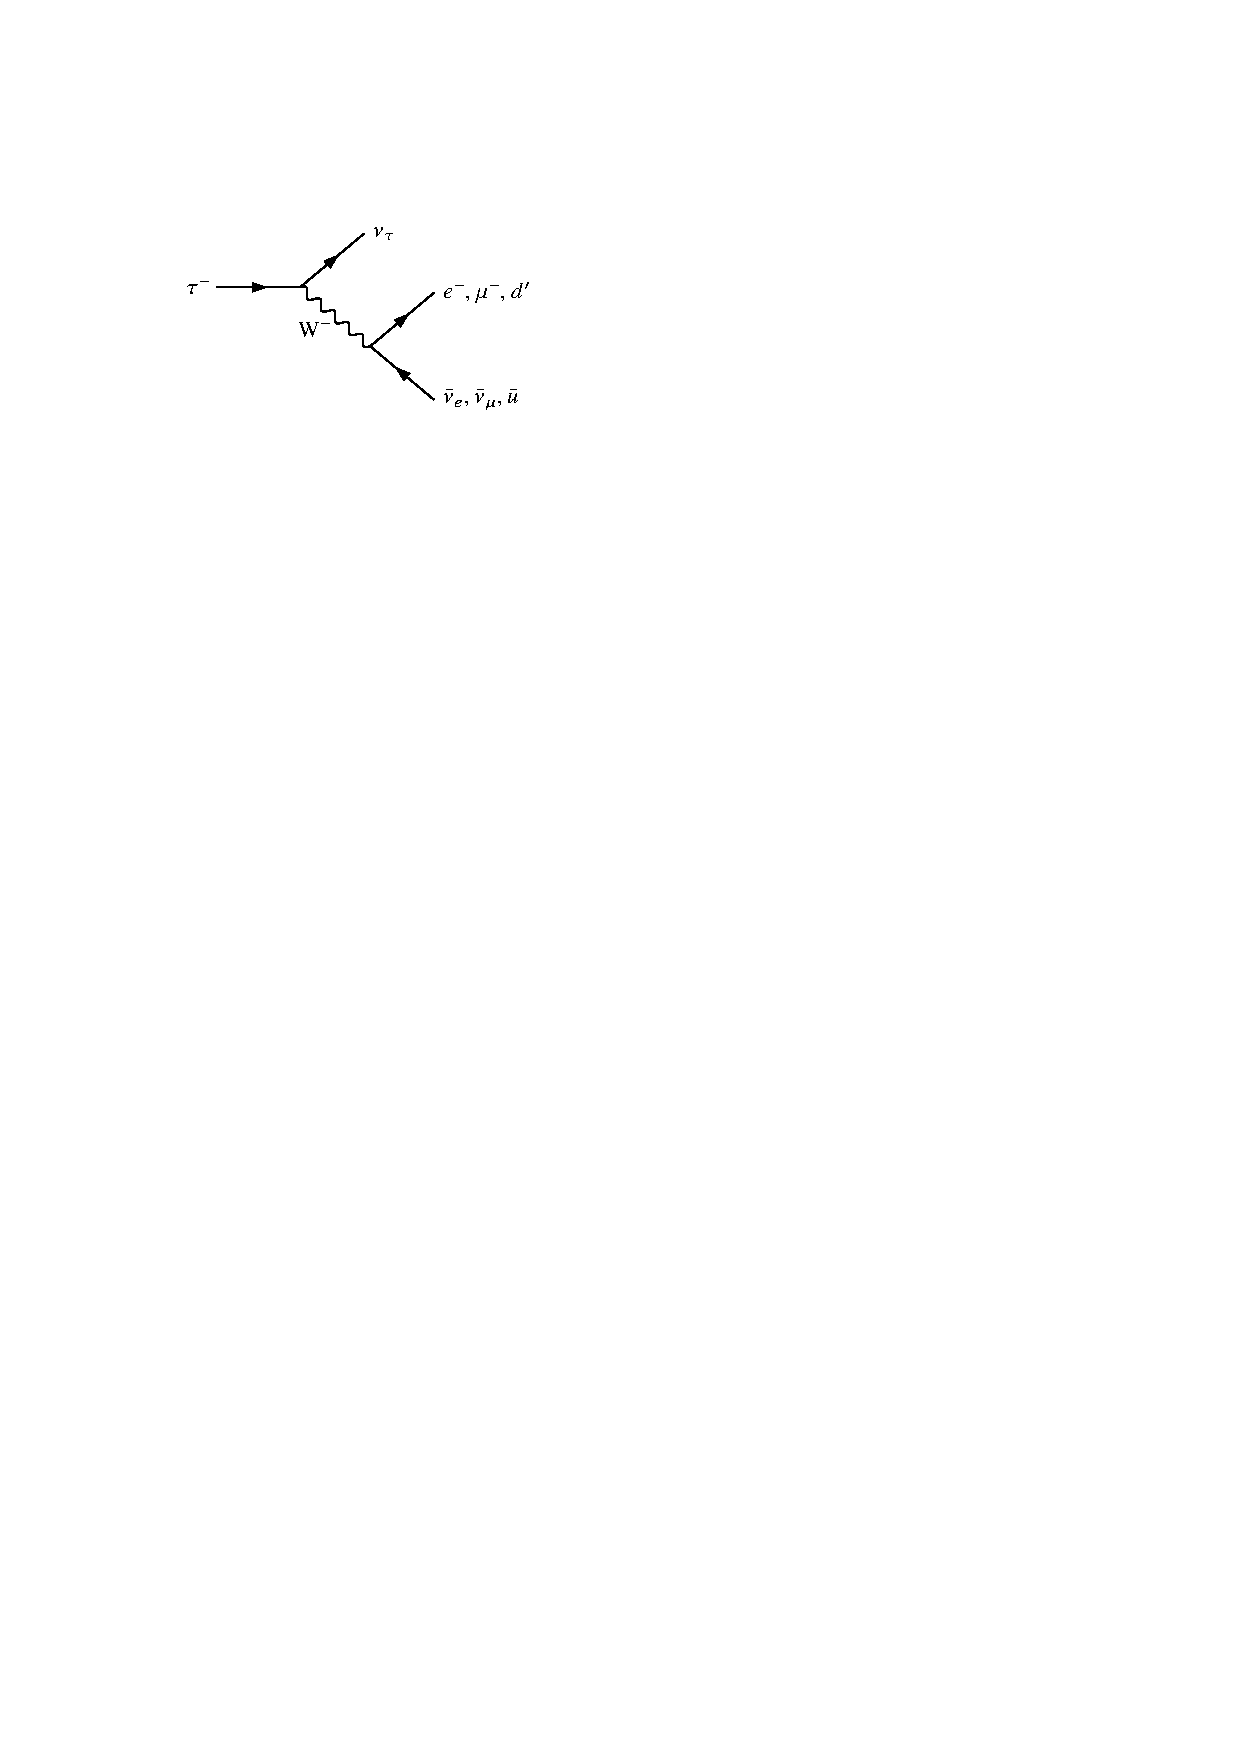
\includegraphics{figs/tauid/tau_decay_feynman}

    \vspace*{3em}
    \subcaption{a}%
    \label{fig:tau_feynman}
  \end{subfigure}\hfill
  \begin{subfigure}[b]{0.47\textwidth}
    \centering

    \begin{overpic}[scale=0.9]{figs/tauid/tau_branching_pie_chart}
      \put (31, 83) {$\pi^- \nu_\tau$}
      \put (-5.5, 45) {$\pi^- \pi^0 \nu_\tau$}
      \put (16, 7) {$\pi^- 2 \pi^0 \nu_\tau$}
      \put (40.5, 2) {$2 \pi^- \pi^+ \nu_\tau$}
      \put (65, 6.5) {$2 \pi^- \pi^+ \pi^0 \nu_\tau$}
      \put (76.5, 15.5) {other}
      \put (70, 77.5) {$e^- \bar{\nu}_e \nu_\tau$}
      \put (88.5, 41.5) {$\mu^- \bar{\nu}_\mu \nu_\tau$}
    \end{overpic}

    \subcaption{}%
    \label{fig:tau_branching_ratios}
  \end{subfigure}
  \caption{Decay and branching ratios of the tau
    lepton. Charge-conjugate decay modes are omitted.}
\end{figure}


\subsubsection{Seed Jet}

Seeded with AntiKt 0.4 jets on TopoClusters at the LC scale.

\subsubsection{Tau Vertex Association}

TJVA

\subsubsection{Track Association}

\cite{duschinger}

\todo[inline]{Make sure to point out the difference between ``tau
  tracks'' and all other tracks.}

\subsubsection{Energy Calibration}

MVA TES

\subsubsection{Electron Veto}
\subsubsection{Tau Identification}

\subsection{Missing Transverse Energy}%
\label{sec:atlas_met}


%%% Local Variables:
%%% mode: latex
%%% TeX-master: "../../phd_thesis"
%%% End:
